\chapter{iSyn: fragment-based drug design}
\label{isyn}

Generating \textit{de novo} ligands from molecular fragments can eliminate the diversity limit of compound repositories and lead to the discovery of novel drugs. State-of-the-art fragment-based drug design (FBDD) tools tend to produce oversized compounds with only moderate potency. Worse, these tools require a long execution time in days.

We present iSyn, a WebGL-based tool for interactive FBDD. It features an evolutionary algorithm that automatically designs novel ligands with drug-like properties and synthetic feasibility using click chemistry. iSyn interfaces with our popular and fast molecular docking engine idock, substantially reducing the evaluation and ranking time of drug candidates. Inspired by our user friendly and high-performance WebGL visualizer iview, our iSyn also implements a tailor-made interactive visualizer to aid novel drug design. To illustrate the utility of iSyn in generating novel ligands \textit{ex nihilo}, we designed predicted inhibitors of two important drug targets, which are RNA editing ligase 1 (REL1) from Trypanosoma brucei, the etiological agent of African sleeping sickness, and cyclin-dependent kinase 2 (CDK2), a positive regulator of eukaryotic cell cycle progression. Results show that iSyn managed to significantly enhance the predicted binding affinity of the best generated ligand by more than 3 orders of magnitude in potency.

iSyn can effectively generate promising compounds with desired potency and molecular mass, and hopefully supplement the efforts of medicinal chemists. iSyn is freely available at http://istar.cse.cuhk.edu.hk/iSyn.tgz.

This was a collaborative project with Chun Ho Chan and Hei Lun Cheung from Department of Computer Science and Engineering, Chinese University of Hong Kong. It was published in the \textit{Proceedings of the 2014 Conference Companion on Genetic and Evolutionary Computation Companion (GECCO)} on 12 July 2014 \citep{1409} and in the \textit{Proceedings of the 18th International Conference on Information Visualisation (IV)} on 15 July 2014 \citep{1387}.

\section{Background}

Given a pharmacological protein of therapeutic interest, protein-ligand docking tries to discover promising ligands out of existing compound databases. The diversity of its outcome is apparently limited by the diversity of the database. In other words, docking is likely to fail if the selected database contains no promising ligands for that particular protein. Hence constructing \textit{de novo} ligands from molecular fragments has now become a hot research topic.

FBDD, though displaying a high chance of discovering novel drugs, is indeed rather challenging because the number of chemically feasible, drug-like molecules has been estimated to be in the order of 10\textsuperscript{60} to 10\textsuperscript{100} \citep{1104}, from which the most promising candidates have to be selected and synthesized. Hence, rather than systematic construction and evaluation of each individual compound, \textit{in silico} FBDD methods rely on the principle of local optimization, which guarantees fast convergence but does not necessarily lead to globally optimal solutions. As a result, most FBDD algorithms are non-deterministic, and feature some extent of stochastic structural optimization.

Recent years have seen a prosperity of FBDD tools, such as LEA3D \citep{1223}, MORPH \citep{365}, GARLig \citep{471}, LigBuilder 2 \citep{749}, AutoT\&T \citep{780}, LiGen \citep{1328,1495}, AutoGrow \citep{466,1354}, AutoClickChem \citep{1051}, CrystalDock \citep{954}, LigMerge \citep{1181}, and the works by \citeauthor{1496} \citep{1496,1500}, by \citeauthor{1497} \citep{1497}, and by \citeauthor{1498} \citep{1498}. More can be found in recent reviews \citep{1493,1499}. Meanwhile, FBDD databases have been established, such as e-Drug3D \citep{1125}. Retrospectively, a number of compounds that evolved from fragments have entered the clinic, and the approach is increasingly accepted as an additional route to identifying new ligands in inhibitor design \citep{363,367,472,474,1006}. Notably, FBDD applications have contributed to the development of a number of FDA-approved drugs \citep{363}, demonstrating their usefulness in real life.

In 2009, the AutoGrow algorithm \citep{466} was developed to aid the identification and optimization of predicted ligands in an automatic manner. Although it lacks the insight and intuition which medicinal chemists have, its high degree of automation requires no user interactions beyond the initial setup of fragment libraries and docking parameters. AutoGrow utilizes a genetic algorithm in conjunction with the AutoDock series software \citep{596,595} to add or exchange moieties of known inhibitors so as to improve their predicted binding affinities. AutoGrow 1.0 and 2.0 use AutoDock4 \citep{596} and AutoDock Vina \citep{595}, respectively, for protein-ligand docking and scoring.

In 2011, we were motivated by the desire to design drug candidates in an interactive way under a virtual reality setting, and thus developed a GUI application \citep{1265} that enables certain human interactions by translating and rotating the generated ligand amid the evolutionary process in a semi-automatic manner. Particularly, in a virtual reality environment when users wear a spectacle with special filters on both sides, the disparity between two superimposed molecules creates a perception of depth, leading to visually more appealing identification of intermolecular interactions.

In 2013, AutoGrow 3.0 \citep{1354} was developed to mainly tackle the synthetic feasibility problem since AutoGrow 1.0 and 2.0 often produce compounds that are neither drug-like nor easily synthesizable. To guide ligand optimization, AutoGrow 3.0 uses the rules of click chemistry, which describes chemistry tailored to generate substances quickly and reliably by joining small units together. A click chemistry reaction would typically be modular and give high chemical yields, and its process would preferably have simple reaction conditions and use readily available starting materials and reagents. To achieve this goal, AutoGrow 3.0 interfaces with AutoClickChem \citep{1051} and LigMerge \citep{1181}, with the former performing virtual modification and joining reactions and the latter performing crossover reactions. AutoClickChem \citep{1051} is capable of performing \textit{in silico} click chemistry reactions, ensuring that chemical synthesis is fast, cheap, and comparatively easy for subsequent testing in biochemical assays. LigMerge \citep{1181} is an automated, ligand-based algorithm for systematically swapping the chemical moieties of known ligands to generate novel ligands with potentially improved potency. It has been shown to identify compounds predicted to inhibit peroxisome proliferator-activated receptor gamma, HIV reverse transcriptase, and dihydrofolate reductase with affinities higher than those of known ligands.% FragVLib \citep{1247} is a free tool for performing similarity search across ligand-receptor complexes for identifying binding pockets similar to that of a target receptor of interest.

\section{Motivation}

Although AutoGrow 3.0 represents the state of the art of FBDD, there are some weak points. AutoGrow 3.0 supports few cutting reactions, which could probably lead to the synthesis of compounds that are too large to absorb by human body. Despite Lipinski's Rule of Fives \citep{169} implemented therein to maintain drug-like properties, generated ligands that violate the rules are simply discarded without further decomposition into small moieties. Moreover, it produces a bunch of new ligands in each generation, and relies on AutoDock Vina \citep{595} to evaluate their predicted binding affinity. The docking efficiency starts to become unacceptable when too many ligands are sampled, prohibiting any more exhaustive approaches. Furthermore, the execution of AutoGrow 3.0 depends on a large set of third-party software including MGLTools \citep{596}, Open Babel \citep{968}, AutoDock Vina \citep{595} and NumPy/SciPy. This highly coupled dependency and the lack of an easy-to-use user interface hinder its pragmatic applications for novices.

\section{Objective}

We present iSyn, our WebGL-based solution for computationally synthesizing \textit{de novo} drug compounds with click chemistry support plus additional cutting reactions. iSyn interfaces with our popular and fast protein-ligand docking engine idock \citep{1153}, greatly reducing the time required for computational evaluations of generated ligands by an order of magnitude \citep{1362} as compared to AutoDock Vina \citep{595}, and thus permitting large-scale executions and exhaustive searching. Most importantly, based on our hardware accelerated WebGL visualizer iview \citep{1366} for protein-ligand complex, our iSyn also features a specific variant of iview in order to compose a user friendly interface as well as to inspect intermolecular interactions and aid novel drug design. As for other enhancements, iSyn utilizes the ultrafast shape recognition (USR) algorithm \citep{1379} to deduplicate ligands, and RF-Score-v3 \citep{1647,1433} to predict accurate binding affinity of generated ligands.

\section{Methods}

Figure \ref{isyn:UI} shows the overall user interface of iSyn. The UI is refactored from Twitter's sleek, intuitive and powerful HTML5 template Bootstrap, and hosted by the lightweight event-driven and non-blocking I/O model node.js. The UI comprises, from top to bottom, a logo, a protein input field, a WebGL canvas, some parameter input fields, a summary panel, some usage instructions, and an export button.

\begin{figure}
\begin{center}
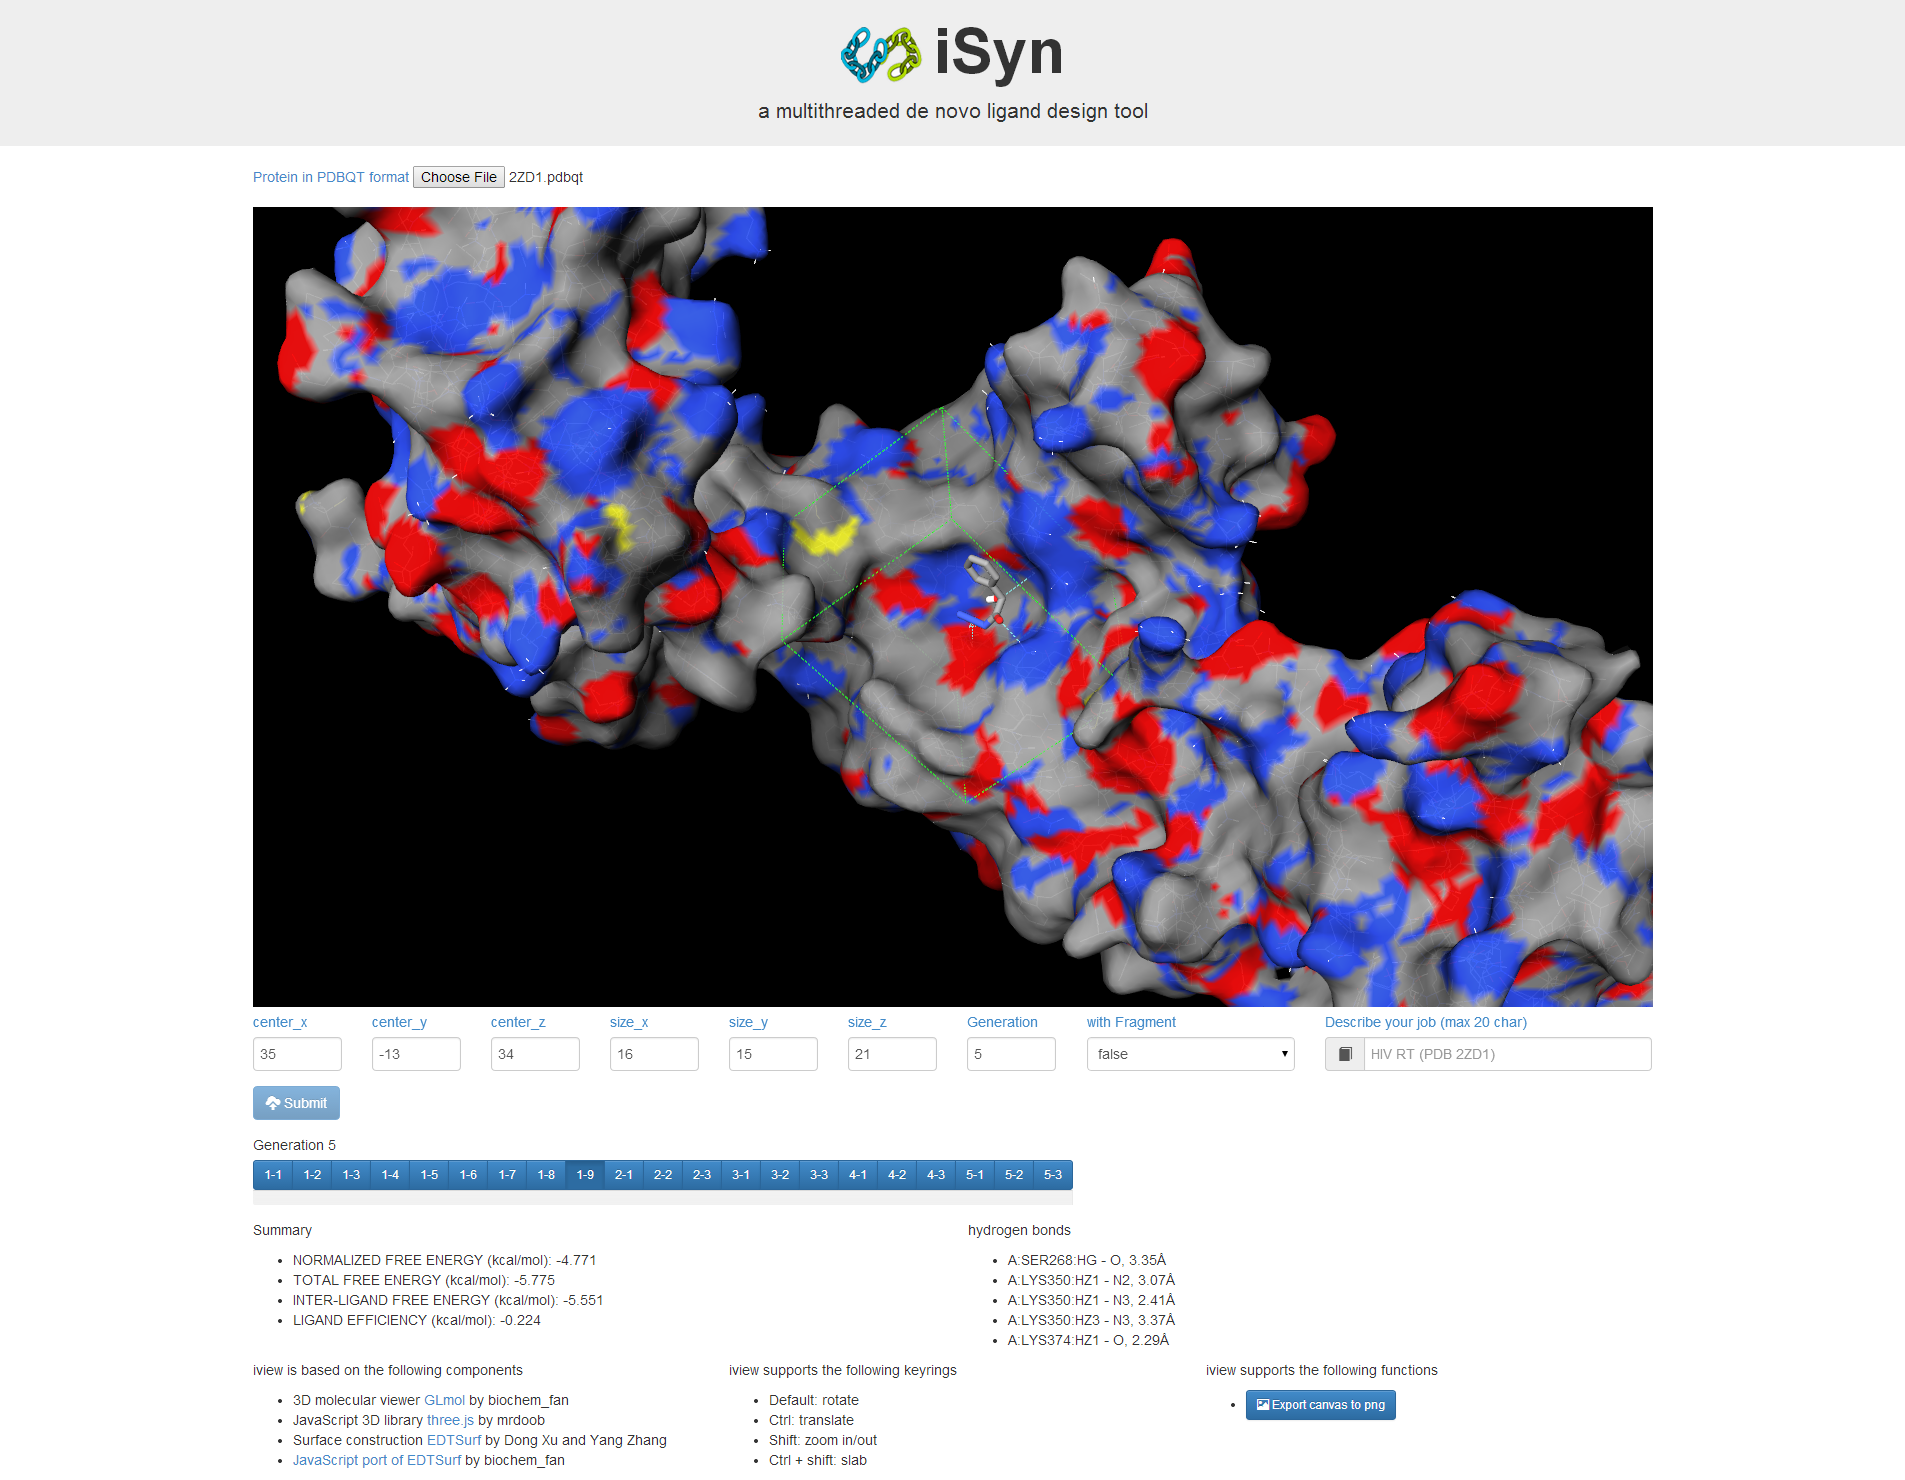
\includegraphics[width=\linewidth]{../isyn/UI.png}
\end{center}
\caption{iSyn user interface.}
\label{isyn:UI}
\end{figure}

In a typical workflow, the user loads a protein target of pharmaceutical interest. The WebGL canvas then automatically renders in real time the protein structure in the representation of lines. Meanwhile, the protein atom coordinates and types are sent to a separate web worker to generate \textit{ad hoc} molecular surface using the EDTSurf algorithm \citep{1297,1350} in background in order to keep the web UI responsive in all time. The protein surface, having been constructed, is automatically applied on top of the line representation. Hence, the user can clearly see the cavities, most likely ligand binding sites, on the protein surface.

The user can then supply the necessary parameters to run iSyn, such as the center and size of the search space, the number of generations of the evolutionary algorithm, a boolean value indicating whether to use the fragment library that accompanies AutoGrow 3.0, and a brief description of the job. The search space is rendered as a dashed cubic box in green. When the user adjusts the values in the input fields, the box is automatically updates accordingly in real time to reflect the actual position. For those optional parameters, we have set up default values so that even novices can get started easily.

Upon clicking the submit button by the user, both the protein structure and the parameters are passed to the backend iSyn executable, immediately commencing the computational synthesis of novel ligands from some initial ligands and the fragments from the fragment library in an exhaustive manner in order to explore as much structural diversity as possible. The fragment library contains acid anhydride, acyl halide, alcohol, thiol, alkene, alkyne, amine, azide, carbonochloridate, carboxylate, epoxide, ester, halide, isocyanate, isothiocyanate, sulfonylazide, and thio acid moieties, and is collected by performing substructure search of the compounds in the ZINC database \citep{532,1178}.

Whenever a population of ligands are generated according to click chemistry reactions, docked against the protein within the binding site, and written to files, the best ligand with the lowest predicted free energy is automatically fetched by the UI in an AJAX fashion using jQuery, a fast, small, yet feature-rich JavaScript library, and visualized in the representation of sticks. Intermolecular putative hydrogen bonds are detected using a cutoff of 3.5Å and rendered as cyan dotted lines.

In the panel beneath the submit button, a number of buttons are dynamically created. Each button represents one conformation of the best ligands in the current generation. In addition, the ligand properties and docking statistics are shown in the summary panel, which is also dynamically updated when a new generation is completed or when the user switches among different ligands by clicking the corresponding button. Having all the relevant information inside one web page, the user can better examine the results in a neat and intact way.

The UI also supports exporting the canvas view to a production-quality image in PNG format via a button. In this way the user can easily capture the canvas without any auxiliary third-party tools.

\subsection{Evolutionary algorithm}

In the first generation, multiple types of click chemistry reactions and structural modifications are applied to the initial ligands selected from the fragment library to synthesize new ligands, where possible duplicates are detected and removed using the USR (Ultrafast Shape Recognition) algorithm \citep{1379}. The generated ligands are then all fed to our popular and fast docking engine idock \citep{1153} to predict their preferred conformations as bound to the protein target, and to prioritize them in the ascending order of their predicted free energy, which reflects the binding affinity. The lower the free energy, the higher the binding affinity. Their conversion factor is derived in \citep{1362}. An extensive benchmark on 12 diverse proteins \citep{1362} has shown that our idock \citep{1153} runs 8.69 to 37.51 times faster than the state-of-the-art AutoDock Vina \citep{595} docking software. The utilization of idock by iSyn promotes the feasibility of large-scale \textit{de novo} drug design and evaluation \textit{in silico}.

The free energy values predicted and sorted by idock are piped to a spreadsheet file in CSV format, which is subsequently parsed by iSyn to retrieve those best ligands with the lowest predicted free energy, i.e. those ligands with the highest predicted binding affinity. To increase the binding affinity prediction accuracy, iSyn provides an alternative option to rescore the docked conformations using our unpublished new version of RF-Score \citep{564}. Then the best ligands in the current generation directly survive into the next generation, and constitute part of the founding ligands. Another part comes from a random selection of the remaining ligands, with the selection probability being proportional to the fitness of a ligand, i.e. its predicted free energy in the case of docking. Our hybrid method, which is essentially a smart combination of the greedy algorithm and the fitness proportionate algorithm, realizes elitism on one hand, while circumvents the risk of over fitting on the other hand.

The evolutionary algorithm either iterates for a number of generations specified by the user, or gets terminated in case of no significant improvement over previous generations.

\subsection{Click chemistry reaction rules}

In iSyn there are four types of operators: addition, mutation, crossover and cutting. They all conform to the requirements of click chemistry. Therefore, the ligands output from iSyn are guaranteed to be chemically synthesizable, making iSyn really pragmatic for medicinal chemistry and computer-aided drug discovery.

The crossover operators are invoked before the addition and mutation operators, while the cutting operators are called at last in order to prevent the generated ligands from becoming oversized.

\subsubsection{Crossover reactions}

iSyn uses the LigMerge algorithm \citep{1181} to perform crossover reactions. Crossover is done by finding the largest common substructure of two parent ligands and matching the different parts of their fragments attached to that common substructure at each common atom, thereby generating multiple child compounds.

\subsubsection{Addition and mutation reactions}

iSyn uses the AutoClickChem algorithm \citep{1051} to perform addition and mutation reactions. The algorithm consists of 30 click chemistry reactions for different functional groups in the reactants, e.g. azide-alkyne and 1,3-dipolar cycloaddition. In order to enumerate the feasibility of performing a particular reaction, ligands are first classified according to their functional groups such as amine, alcohol, azide, etc.

\subsubsection{Cutting reactions}

Through the addition and mutation operators, ligands could possibly ``grow” too large in terms of molecular size, and might therefore lose drug-like properties. For example, if a generated ligand has a molecular mass of over 500 Daltons, it is unlikely to be absorbed inside the human body and thus unlikely to be optimized into a potential drug. In light of this issue, we have implemented four novel cutting operators to break down oversized ligands.

Ozonolysis is the cleavage of an alkene with ozone to form organic compounds where the carbon-carbon double bond is replaced by a double bond to oxygen (Figure \ref{isyn:AlkeneOzonolysis}). The alkene functional group is oxidized with ozone to form aldehydes or ketones, depending on the structure of the ligand under a certain chemical environment. Through this reaction, a ligand containing a carbon-carbon double bond can be broken down into two child ligands.
 
\begin{figure}
\begin{center}
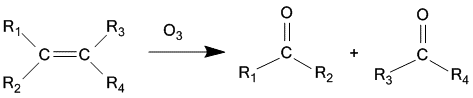
\includegraphics[width=\linewidth]{../isyn/AlkeneOzonolysis.png}
\end{center}
\caption{Ozonolysis of alkene.}
\label{isyn:AlkeneOzonolysis}
\end{figure}

Vigorous oxidation on alkene can form carbolic acid (Figure \ref{isyn:AlkeneOxidation}). While oxidation of alkene gives out aldehydes or ketone, further oxidation gives out carboxylic acid and alcohol as products. Aldehyde can be easily oxidized by all sorts of oxidizing agents. As for ketone, although it has certain resistance to oxidation, it can also be oxidized to carboxylic acid by using strong oxidizing agents such as potassium manganite VII solution. Through this reaction, a ligand containing carbon-carbon double bonds can be broken down into four child ligands.
 
\begin{figure}
\begin{center}
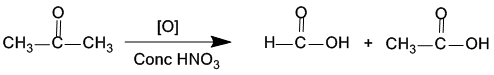
\includegraphics[width=\linewidth]{../isyn/AlkeneOxidation.png}
\end{center}
\caption{Oxidation of alkene to carboxylic acid.}
\label{isyn:AlkeneOxidation}
\end{figure}

Acid anhydrides can react with water to form carboxylic acid (Figure \ref{isyn:AcidAnhydrideReaction}). An acid anhydride has two acyl groups bound to the same oxygen atom. The two acyl groups are derived from the same carboxylic acid. In reverse, the acid anhydride can be broken down into two original carboxylic acids by reacting with water. Through this reaction, a ligand containing two acyl groups bound to the same oxygen atom can be broken down into two child ligands.

\begin{figure}
\begin{center}
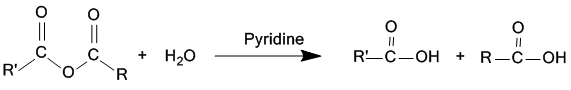
\includegraphics[width=\linewidth]{../isyn/AcidAnhydrideReaction.png}
\end{center}
\caption{Acid anhydride to carboxylic acid.}
\label{isyn:AcidAnhydrideReaction}
\end{figure}

Hydrolysis of ester is the reverse of esterification (Figure \ref{isyn:EsterHydrolysis}), which is a reversible reaction. The reaction is catalyzed by diluted acid, such as diluted hydrochloric acid, and is heated under reflux. As the reaction is reversible, excessive water has to be used. Under such condition, carboxylic acid and alcohol are produced. Through this reaction, a ligand containing ester groups can be broken down into two child ligands.

\begin{figure}
\begin{center}
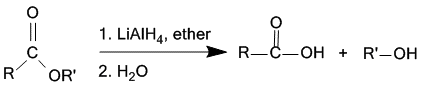
\includegraphics[width=\linewidth]{../isyn/EsterHydrolysis.png}
\end{center}
\caption{Hydrolysis of ester.}
\label{isyn:EsterHydrolysis}
\end{figure}

\subsection{WebGL visualizer}

Perhaps the most vital difference that distinguishes iSyn apart from many other FBDD tools is the availability of a WebGL visualizer, which is not only user friendly, but also of high performance. Unlike Java applet-based visualizers that require Java installation and depend on software rendering which is slow on large display areas and prevents detailed inspection of the structure, iSyn's WebGL visualizer is refactored from our iview \citep{1366} using three.js as its primary 3D engine with anti-aliasing support, and benefits from GPU hardware acceleration. Because of no dependency on any third-party browser plugins, our visualizer demonstrates excellent portability and usability.

The visualizer uses EDTSurf \citep{1297,1350}, a fast algorithm to generating triangulated macromolecular surfaces by Euclidean distance transform, to construct and render in real time four representations of protein surface, namely Van der Waals surface, solvent excluded surface, solvent accessible surface and molecular surface. Note that molecular surface is indeed solvent excluded surface, but EDTSurf uses different ways to derive them.

The visualizer supports certain kinds of user interactions including rotation, translation, zooming and changing slab with mouse or hand touch manipulation. It is functional not only on desktop computers, but also on mobile devices such as Android phones and tablets that support WebGL.

It is noteworthy to point out that iSyn performs all sorts of parsing and rendering in the client browser, ensuring the data privacy and confidentiality are retained.

\section{Results and discussion}

Thus far there are no well-established systematic evaluation metrics and benchmarks for FBDD tools, therefore selected examples are often used for testing purpose, as was the case in AutoGrow \citep{466,1354}. To demonstrate the utility of our iSyn in generating novel ligands \textit{ex nihilo}, we designed predicted inhibitors of two important drug targets, which are RNA editing ligase 1 (REL1) from Trypanosoma brucei, the etiological agent of African sleeping sickness, and cyclin-dependent kinase 2 (CDK2), a positive regulator of eukaryotic cell cycle progression.

We evaluated and compared our iSyn and the state-of-the-art AutoGrow 3.0 from the perspectives of the lowest predicted free energy obtained and the program execution time on a Linux server equipped with 2 Xeon E5-2670 @ 2.6GHz and 128GB ECC DDR3.

\subsection{Inhibitors of Trypanosoma brucei RNA editing ligase 1}

As TbREL1 is crucial for the survival of the Trypanosoma brucei parasite, it has been the target of several drug discovery projects over recent years.

PDB entry 1XDN was used. 75 initial ligands were chosen as input from the MW250 subset of the AutoGrow 3.0 fragment library by randomly picking 5 fragments from each of the 15 categories.

AutoGrow 3.0 was run for 2 days and 10 hours for 17 generations, and the best resultant compound had predicted free energy of -12.7 kcal/mol.

iSyn was run for 6 hours and 40 minutes for 2 generations, and the best resultant compound, 2\_1314\_1, had predicted free energy of -14.176 kcal/mol, with as many as 17 putative hydrogen bonds (Figure \ref{isyn:1XDN}).

\begin{figure}
\begin{center}
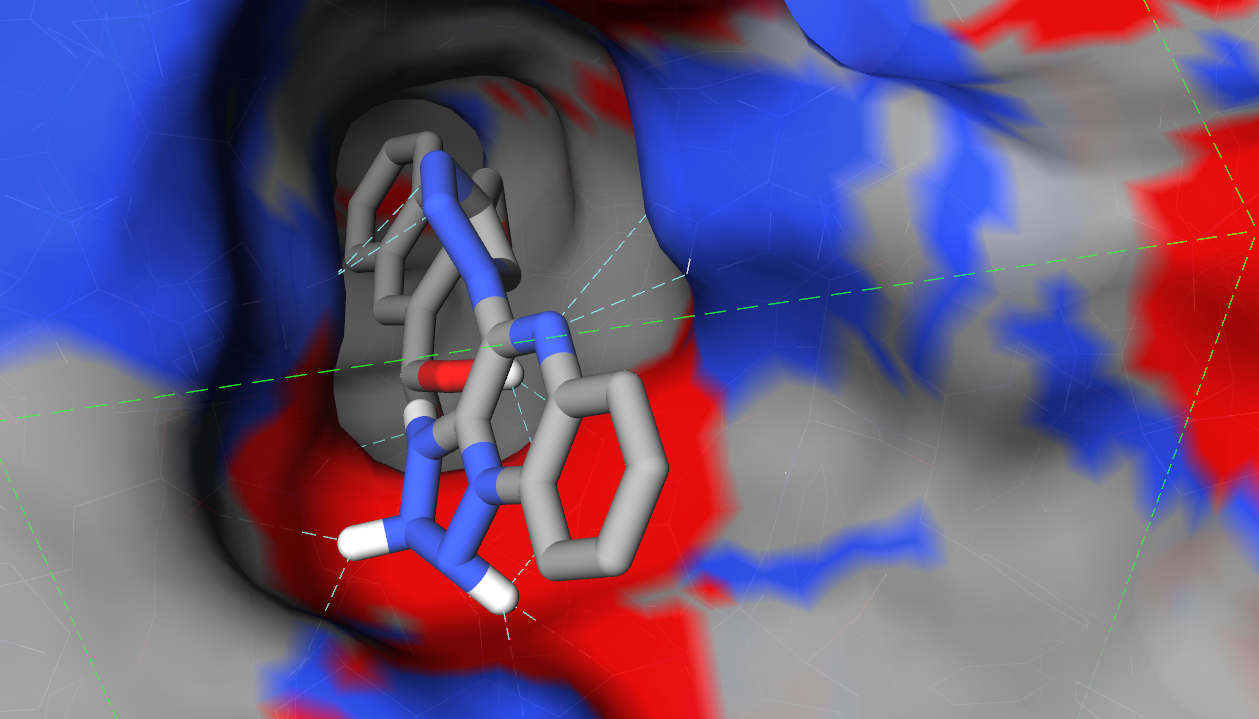
\includegraphics[width=\linewidth]{../isyn/1XDN.png}
\end{center}
\caption{TbREL1 in complex of 2\_1314\_1.}
\label{isyn:1XDN}
\end{figure}

iSyn is capable of tracking the synthetic path of child ligands from their ancestors. Figure \ref{isyn:2_1314_1} shows the evolutionary steps taken to produce 2\_1314\_1, whose starting ligand had predicted free energy of -9.671 kcal/mol. After 2 generations, the best ligand 2\_1314\_1 had 4.505 kcal/mol lower predicted free energy. Since the value is in logarithmic scale, it effectively translates to 2016 fold increase in drug potency. In other words, a small concentration of the 2\_1314\_1 molecule would be sufficient to modulate the biological function of the TbREL1 target.

\begin{figure}
\begin{center}
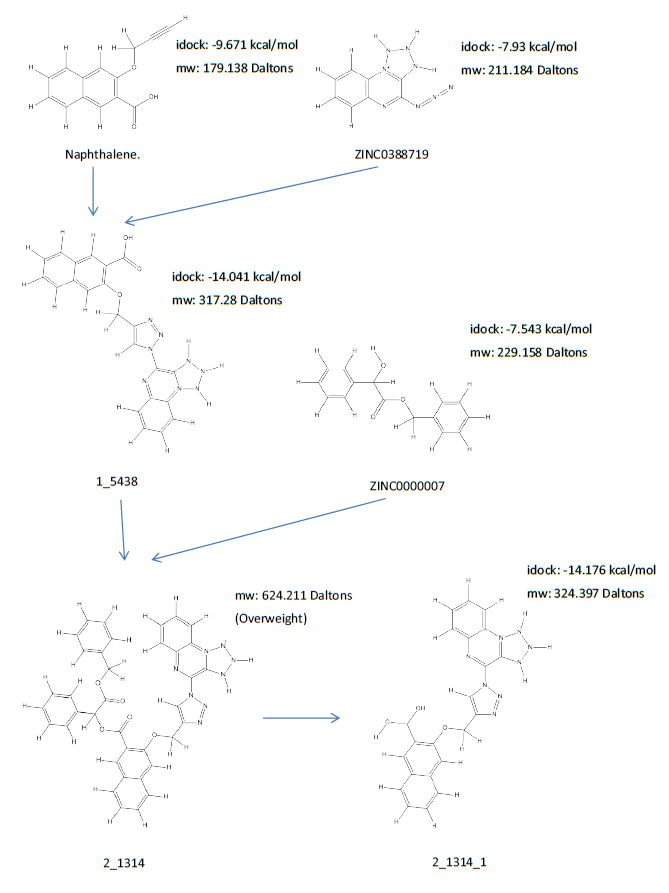
\includegraphics[width=\linewidth]{../isyn/2_1314_1.png}
\end{center}
\caption{The evolutionary steps taken to generate 2\_1314\_1.}
\label{isyn:2_1314_1}
\end{figure}

It can also be seen that its parent ligand, 2\_1314, had a molecular mass of as large as 624.211 Daltons, which is unlikely to be optimized into potent drugs. Thanks to our four novel cutting operators, it got broken down and resulted in the ever best ligand. This demonstrates the helpfulness of our newly-implemented cutting operators with click chemistry support.

In another run of iSyn with the same target, 20,392 initial ligands from the MW250 subset were used as input. iSyn was run for 2 days and 4 hours for 3 generations, and the best resultant compound, Gen2\_m24517, had predicted free energy of -15.393 kcal/mol. This indicates that iSyn was able to generate even better ligands when more generations were achieved. Figure \ref{isyn:Gen2_m24517} shows the evolutionary steps taken to generate Gen2\_m24517.

\begin{figure}
\begin{center}
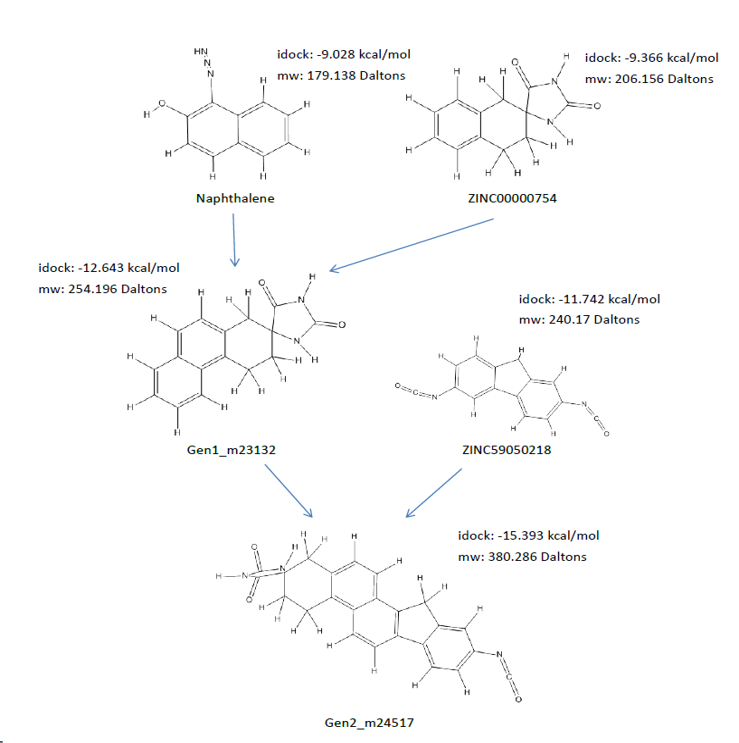
\includegraphics[width=\linewidth]{../isyn/Gen2_m24517.png}
\end{center}
\caption{The evolutionary steps taken to generate Gen2\_m24517.}
\label{isyn:Gen2_m24517}
\end{figure}

\subsection{Inhibitors of cyclin-dependent kinase 2}

CDK2 is a member of the cyclin-dependent kinase family that are potential therapeutic targets for oncology. Inhibition of CDK2 may represent a therapeutic strategy for prevention of many cell cycle related diseases.

PDB entry 1JSV was used. Likewise, a number of ligands were chosen randomly from the fragment library to act as initial ligands.

iSyn was run for 11 hours and 20 minutes for 4 generations, and the best resultant compound had predicted free energy of -11.345 kcal/mol, with 9 putative hydrogen bonds (Figure \ref{isyn:1JSV}). For comparison, its starting ligand had predicted free energy of only -5.607 kcal/mol.

\begin{figure}
\begin{center}
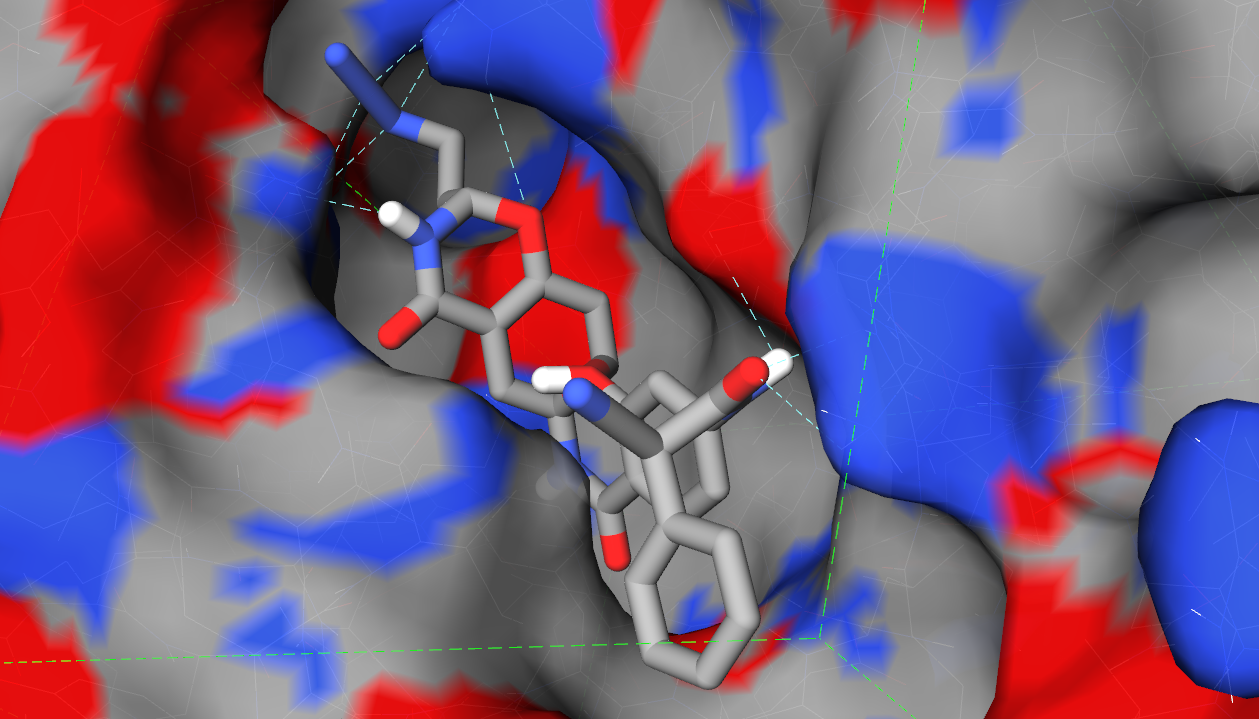
\includegraphics[width=\linewidth]{../isyn/1JSV.png}
\end{center}
\caption{CDK2 (PDB: 1JSV) in complex of the best ligand.}
\label{isyn:1JSV}
\end{figure}

In another run of iSyn with the same target, PDB entry 1PXM was used. We would like to test whether iSyn could produce consistent results given different PDB entries of the same protein.

iSyn was run for 14 hours and 30 minutes for 5 generations, and the best resultant compound had predicted binding affinity of -14.071 kcal/mol, with 12 putative hydrogen bonds (Figure \ref{isyn:1PXM}).
 
\begin{figure}
\begin{center}
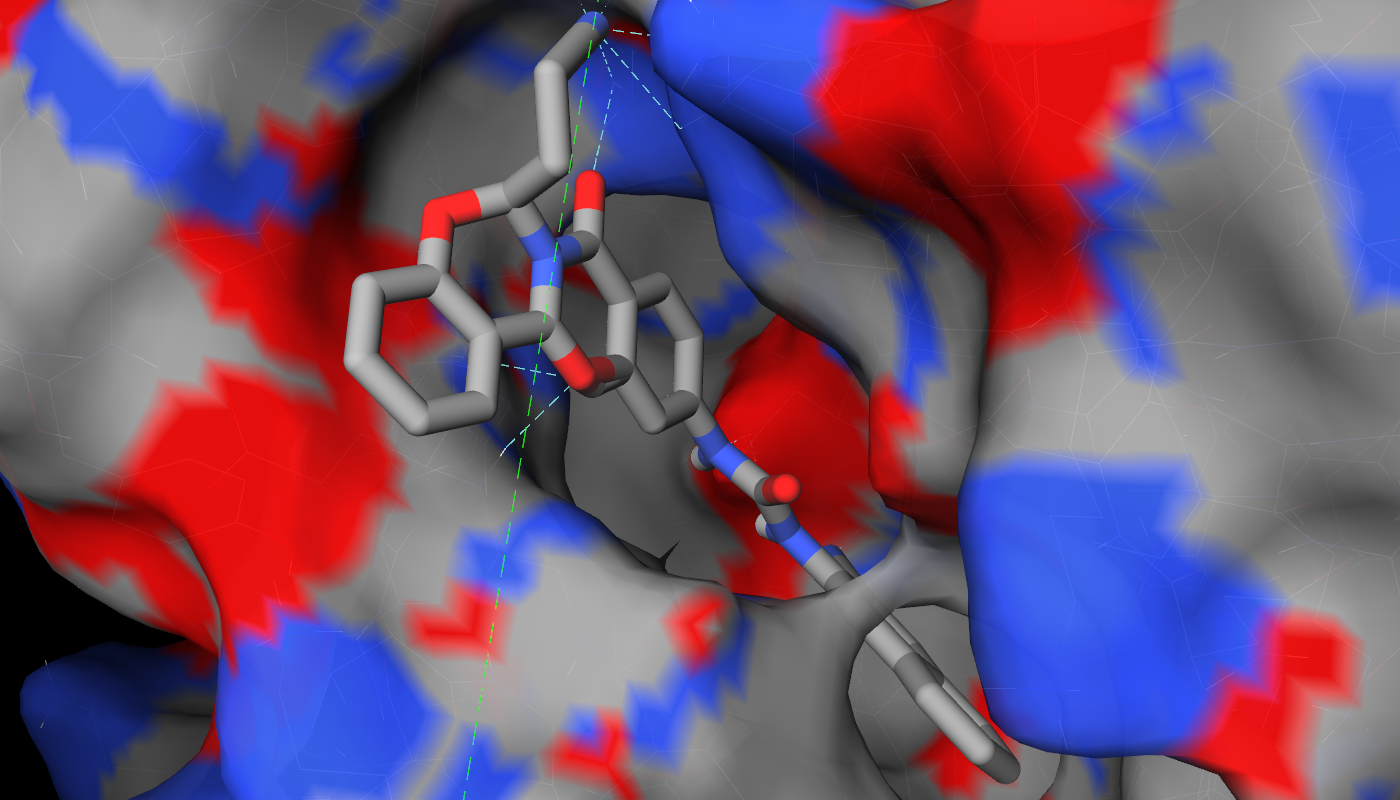
\includegraphics[width=\linewidth]{../isyn/1PXM.png}
\end{center}
\caption{CDK2 (PDB: 1PXM) in complex of the best ligand.}
\label{isyn:1PXM}
\end{figure}

Obviously, the best ligand obtained in this example is better than the one obtained in the previous example. This could be due to several reasons. The major reason is most likely the stochastic nature of the evolutionary algorithm. Different optimization runs typically lead to different results. Another reason is the possible conformational differences in the two protein-ligand complex entries, which could affect intermolecular binding. A third reason is the difference in the center and size of the binding site. Nevertheless, in both examples the best ligand still had predicted free energy lower than -11 kcal/mol, indicating that iSyn managed to produce very potent ligands in both cases.

In another run of iSyn with the same target, PDB entry 1PF8 was used. Its experimentally measured binding affinity is $K_i$=31nM. Within just 4 hours and 10 minutes, iSyn generated the best ligand with predicted free energy of -14.4 kcal/mol, which translates to 27pM in potency. This is over one thousand times more potent than the crystal ligand.

\section{Conclusions}

Although \textit{in silico} fragment-based drug design (FBDD) represents a promising approach to complement structure-based virtual screening, few FBDD tools show satisfactory performance in terms of achieved potency and computational resources.

In this study we have presented iSyn, our WebGL-based solution for computationally synthesizing \textit{de novo} drug compounds with click chemistry support plus additional cutting reactions. iSyn is a methodological mixture of ligand duplication by USR \citep{1379}, four new cutting reactions, efficient docking by idock \citep{1153}, accurate rescoring by RF-Score-v3, fitness proportionate selection and intelligent termination in genetic algorithm, and WebGL visualization with molecular surface. Various test cases on TbREL1 and CDK2 have proved its strength in finding candidate drug compounds within a reasonable time. We hope that the iSyn can pragmatically assist medicinal chemists in optimizing candidate compounds and designing novel drugs.

\section{Availability}

iSyn is written in C++, Python, HTML5 and JavaScript. It is free and open source, available at http://istar.cse.cuhk.edu.hk/iSyn.tgz. It has been tested successfully on both Linux and Windows.

\section{Future works}

There are some major weak points about iSyn, though. iSyn requires ligands in PDB format to perform the genetic operators, but it requires PDBQT format to perform docking and scoring. So every generated ligand must undergo PDB-to-PDBQT conversion, which incurs substantial overhead. Moreover, one user recently found a bug in iSyn that after a cutting reaction, iSyn discarded the large fragment and retained the small one, which was subsequently discarded again.

We are developing a new project called igrow to directly manipulate ligands in PDBQT format. A further attempt would be to incorporate igrow into idock to better speed up the docking process. It is also inspiring to design multitarget ligands \citep{366,1497}.

\chapterend
